\documentclass[12pt]{article}
\usepackage{amsmath}
\usepackage[utf8]{inputenc}
\usepackage[russian]{babel}
\usepackage{color}
\usepackage[usenames,dvipsnames]{xcolor}
\usepackage{graphicx}

\title{Математический анализ. Контрольная работа №3 - Роман Гафиятуллин (192001-04)}
\author{Роман Гафиятуллин\\ БГУИР}
\begin{document}
	\begin{titlepage}
		\begin{center}
			{\Large Математический анализ. \\ Контрольная работа №3 \\ Роман Гафиятуллин (192001-04)}
		\end{center}
	\end{titlepage}
	%%%%%%%%%%%%%%%%%%%%%%%%%%%%%%%%%%%%%%%%%%%%%%%%%%%%%%%%%%%%%%%%%%%%%%%%%%%%%%%%%%%%%%%%%%%%%%%%%%%%%%%%%%%%%%
	\clearpage
	\paragraph{04-3.1} Найти неопределенные интегралы. В случаях а), б), в) результат проверить дифференцированием. \\
	\begin{description}
		\item[а)] \ensuremath{
			\int \frac{d x}{sin ^2 x (2 ctg x + 1)} =\\
			= \frac{1}{sin ^2 x ( 2 ctg x + 1 )} = \\
			\textcolor{Cyan}{// \frac{1}{sin x} = csc x } \\
			= \frac{csc ^2 x}{2 ctg x + 1} = \\
			\textcolor{Cyan}{// u = 2 ctg x + 1} \\
			\textcolor{Cyan}{// du = - 2 csc ^2 (x) dx} \\
			= -\frac{1}{2} \int \frac{1}{u} du = \\
			\textcolor{Cyan}{ \int \frac{1}{u} = log(u) } \\
			= -\frac{log(u)}{2} + const = \\
			\textcolor{Cyan}{// u = 2 ctg x + 1 } \\
			= {\bf -\frac{1}{2} log ( 2 ctg x + 1 ) + const }
		}
		\item[б)] \ensuremath{
			\int \frac{x arccos x}{\sqrt{1 - x ^2}}dx = \\
			= \int x \sqrt{1 - x ^2} arccos(x) dx = \\
			\textcolor{Cyan}{// u = arccos(x) } \\
			\textcolor{Cyan}{// du = - \frac{1}{\sqrt{1 - x ^2}}dx } \\
			= \int -u sin ^2 (u) cos (u) du = \\
			= - \int u sin ^2 (u) cos(u) du = \\
			\textcolor{Cyan}{// sin ^2 (u) = 1 - cos ^2 (u) } \\
			= - \int cos(u) ( 1 - cos ^2 (u) ) du = \\
			= \int ( u \cdot cos(u) - u \cdot cos ^3 (u) ) du = \\
			= \int u \cdot cos ^3 (u) du - \int cos (u) du = \\
			\textcolor{Cyan}{// \int f dg = f g - \int g df} \\
			\textcolor{Cyan}{// // f = u, dg = cos(u)du } \\
			\textcolor{Cyan}{// // df = du, g = sin(u) } \\
			= -u sin(u) + \int sin(u) du + \int u \cdot cos ^3 (u) du = \\
			\textcolor{Cyan}{// u \cdot cos ^2 (u) = \frac{(cos(2 u) + 1)}{2} } \\
			= -u sin(u) + \int sin(u) du + \frac{1}{2} \int u \cdot cos(u) (cos(2u) + 1) du = \\
			= -u sin(u) + \int sin(u) du + \frac{1}{2} \int (u \cdot cos(u) + u \cdot cos(2 u) cos(u) du) = \\
			\textcolor{Cyan}{// cos(\alpha)cos(\beta) = \frac{1}{2}(cos(\alpha - \beta) + cos(\alpha + \beta)) } \\
			\textcolor{Cyan}{// \alpha = u, \beta = 2u} \\
			= -u sin(u) + \int sin(u) du + \frac{1}{4} \int (u \cdot cos(u)+ u \cdot cos(3u)) du + \frac{1}{2} \int u \cdot cos(u) du = \\
			= -u sin(u) + \int sin(u) du + \frac{1}{4} \int u \cdot cos(u) du + \frac{1}{4} \int u \cdot cos(3u) du + \frac{1}{2} cos(u) du = \\
			\textcolor{Cyan}{// \int f dg = f g - \ g df } \\
			\textcolor{Cyan}{// f = u, dg = cos(3u) du} \\
			\textcolor{Cyan}{// df = du, g = \frac{1}{3} sin (3u)} \\
			= -u sin(u) + \frac{1}{12} u sin(3u) - \frac{1}{12} \int sin(3u) du + \int sin(u)du + \\
			 + \frac{1}{2}u \cdot cos(u) du + \frac{1}{4}\int u \cdot cos(u) du = \\
			\textcolor{Cyan}{// s = 3u, ds = 3du} \\
			= - \frac{1}{36} \int sin(s)ds - u sin(u) + \frac{1}{12} u sin(3u) + \int sin(u) du + \\
			 + \frac{1}{2} \int u \cdot cos(u) du + \frac{1}{4} \int u \cdot cos(u) du = \\
			= \frac{cos(s)}{36} - u sin(u) + \frac{1}{12} u sin(3u) + \int sin(u) du + \\
			 + \frac{1}{2} \int u \cdot cos(u) du + \frac{1}{4} \int u \cdot cos(u) du = \\
			\frac{cos s}{36} - \frac{3}{4} u sin(u) + \frac{1}{12} u sin (3u) - \\
			 - \frac{1}{4} \int sin(u) du + \int sin(u) du + \frac{1}{2} u cos(u) du = \\
			= \frac{cos s}{36} - \frac{1}{4} u sin(u) + \frac{1}{12} u sin (3u) + \frac{cos u}{4} -
			 - \frac{1}{2} \int sin (u) du + \int sin(u) du = \\
			= \frac{cos s}{36} - \frac{1}{4} u sin (u) + \frac{1}{12} u sin (3u) + \\
			 + \frac{cos(u)}{4} - \frac{1}{2} \int sin(u) du + \int sin(u) du = \\
			= \frac{cos(s)}{36} - \frac{1}{4} u sin (u) + \frac{1}{12} u sin (3u) - \frac{cos u}{4} + const = \\
			\textcolor{Cyan}{// s = 3u } \\
			= -\frac{1}{4} u sin (u) + \frac{1}{12} u sin (3u) - \frac{cos u}{4} + \frac{1}{36} cos(3u) + const = \\
			\textcolor{Cyan}{// u = arccos(x)} \\
			= {\bf \frac{1}{9} (x ^3 - 3(1 - x ^2)^{\frac{3}{2}} \cdot arccos(x) - 3 x ) + const }
		}
		\item[в)] \ensuremath{
			\int \frac{d x}{x ^3 - x ^2 + 2 x - 2} = \\
			= \frac{1}{6}(-log (x ^2 + 2) + 2 log(1 - x) - \sqrt{2} \cdot arctg(\frac{x}{\sqrt{2}})) + const = \\
			= \frac{1}{3} \int \frac{-x - 1}{x ^2 + 2} dx  + \frac{1}{3} \int \frac{1}{x - 1} dx = \\
			= -\frac{1}{3} \int \frac{1}{x ^2 + 2} dx - \frac{1}{3} \int \frac{x}{x ^2 + 2} dx
			 + \frac{1}{3} \int \frac{1}{x - 1}dx = \\
			= -\frac{1}{6} log (x ^2 + 2) + \frac{1}{3}log(x - 1) - \frac{ arctg \frac{x}{\sqrt{2}} }{ 3 \sqrt{2} } + const = \\
			{\bf \frac{1}{6}( -log (x ^2 + 2) + 2 log (1 - x) - \sqrt{2} arctg\frac{x}{\sqrt{2}} ) + const }
		}
		\item[г)] \ensuremath{
			\int \frac{x + \sqrt[3]{1 + x}}{\sqrt{1 + x}} dx = \\
			= {\bf \frac{2}{15} \sqrt{x + 1} ( 5 x + 9 \sqrt[3]{x + 1} - 10 ) + const }
		}
		\item[д)] \ensuremath{
			\int sin ^2 x \cdot cos ^2 x dx = \\
			= {\bf \frac{1}{32}(4 x - sin(4 x)) + const }
		}
	\end{description}

	%%%%%%%%%%%%%%%%%%%%%%%%%%%%%%%%%%%%%%%%%%%%%%%%%%%%%%%%%%%%%%%%%%%%%%%%%%%%%%%%%%%%%%%%%%%%%%%%%%%%%%%%%%%%%%
	% \clearpage
	\paragraph{04-3.2} Вычислить определенные интегралы.
	\\\\
	\ensuremath{
		\int_{0}^{1} \frac{5 x + 1}{x ^2 + 2 x + 1} dx = \\
		= \frac{4}{x + 1} + 5 log( x + 1 ) = \\
		= 2 + 5 log(2) - ( 4 + 5 log (1) )  \\
		= {\bf 5 log(2) - 2 \approx 1.465 }
	}
	
	%%%%%%%%%%%%%%%%%%%%%%%%%%%%%%%%%%%%%%%%%%%%%%%%%%%%%%%%%%%%%%%%%%%%%%%%%%%%%%%%%%%%%%%%%%%%%%%%%%%%%%%%%%%%%%	
	% \clearpage
	\paragraph{04-3.3} Вычислить площадь фигуры, ограниченной заданными линиями. Сделать чертеж.
	\\\\
	\ensuremath{
		x ^2 - 6 y = 0 \\
		x + 6 y - 12 = 0
	}
	\\
	\\
	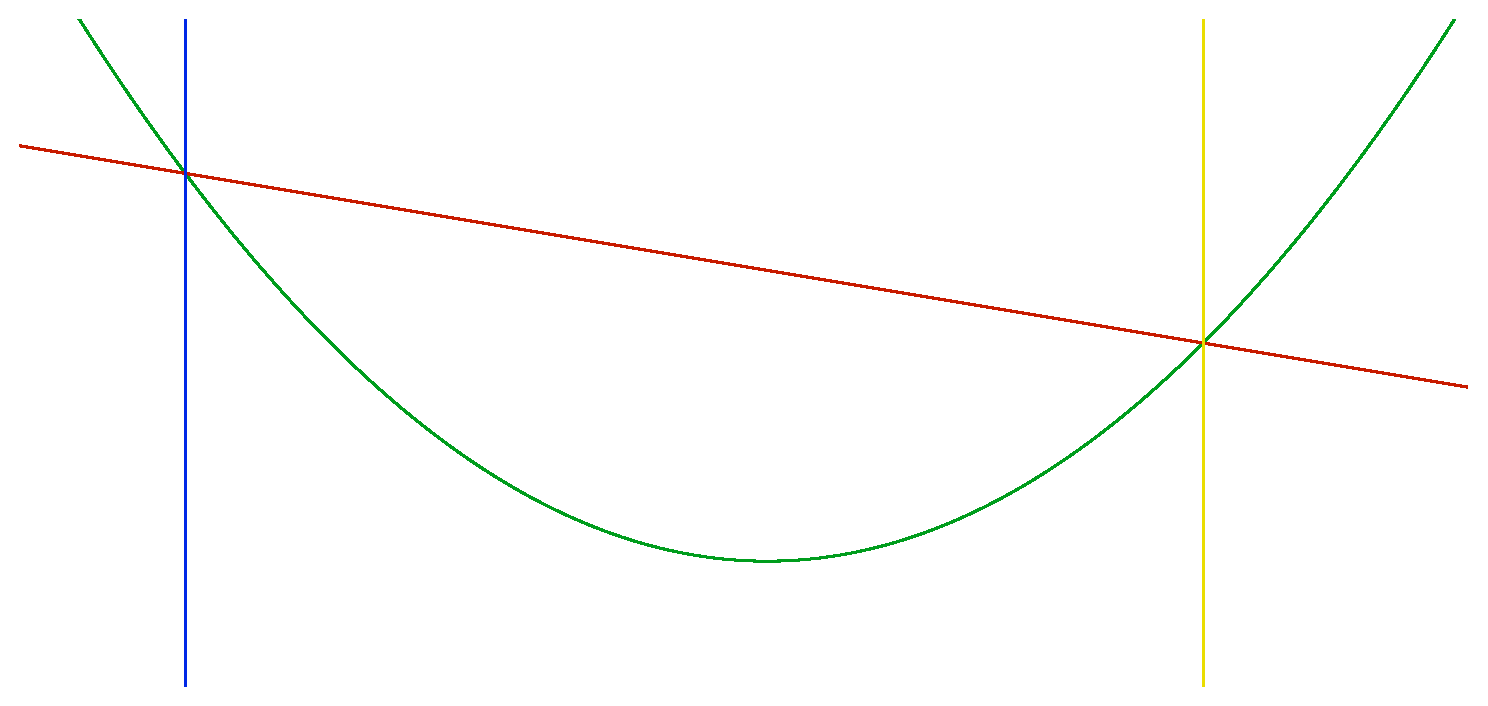
\includegraphics[width=200px,height=100px]{RG-Uni-Calculus-Reference_Work_3-04-1-3.eps}
	\\
	\ensuremath{
		\textcolor{Blue}{ x = -4 };
		\textcolor{Red}{ y = 2 - \frac{x}{6} }; \\
		\textcolor{Yellow}{x = 3 };
		\textcolor{Green}{ y = \frac{x ^2}{6} };
	}
	\\\\
	Площадь образованной фигуры: \\
	\ensuremath{
		\int_{\textcolor{Blue}{-4}}^{\textcolor{Yellow}{3}} \textcolor{Red}{ 2 - \frac{x}{6} } - \textcolor{Green}{ \frac{x ^2}{6} } dx =\\
		= \int_{-4}^{3} - \frac{x ^3}{18} - \frac{x ^2}{12} + 2 x = \frac{343}{36} \approx 9.52778 \\
	}

	%%%%%%%%%%%%%%%%%%%%%%%%%%%%%%%%%%%%%%%%%%%%%%%%%%%%%%%%%%%%%%%%%%%%%%%%%%%%%%%%%%%%%%%%%%%%%%%%%%%%%%%%%%%%%%
	% \clearpage
	\paragraph{04-3.4} Вычислить приближенное значение определенного интеграла \ensuremath{\int_{b}^{a} f(x) dx} с помощью формулы Симпсона, разбив отрезок инегрирования на 10 частей. Все вычисления проводить с округлением до третьего десятичного знака.
	\\\\
	\ensuremath{\int_{0}^{10}\sqrt{x ^3 + 5} dx}
	\\

	%%%%%%%%%%%%%%%%%%%%%%%%%%%%%%%%%%%%%%%%%%%%%%%%%%%%%%%%%%%%%%%%%%%%%%%%%%%%%%%%%%%%%%%%%%%%%%%%%%%%%%%%%%%%%%
	% \clearpage
	\paragraph{04-3.5} Вычислить несобственный интеграл или доказать, что он расходится.
	\\\\
	\ensuremath{
		\int_{0}^{1} \frac{x dx}{\sqrt{1 - x ^2} } = \\
		= \lim_{b \to 1-0} \int_{0}^{b} \frac{x \cdot dx}{\sqrt{1 - x}} = \\
		= - \lim_{b \to 1-0} \sqrt{1 - x^2}|_{0}^{b} = \\
		= - ( 0 - 1 ) = {\bf 1 }
	}
\end{document}

